\DeclareSong{The Mute}{Radical Face}{The Family Tree: The Branches}[2]
\vskip -1em
\intro{C\pause F\rep{3}\Pause G\pause G\susfour}
\begin{strophe*}
  \chord[c]{Am}Well, as a child I mostly \chord[c]{F}spoke inside my \chord[c]{C}head

  \chord[c]{Am}I had conversations with the \chord[c]{F}clouds, the dogs, the \chord[c]{C}dead

  \chord[c]{Am}And they thought me broken, that my \chord[c]{F}tongue was coated \chord[c]{C}lead

  But I just \chord[c]{G}couldn't make my \chord[c]{F}words make sense to \chord[c]{Am}them

  If you only \chord[c]{G}listen with your \chord[c]{F}ears... I can't get \chord[c]{C}in
\end{strophe*}
\vskip 0.6em
\begin{strophe*}
  \chord[c]{Am}And I spent my evenings pulling \chord[c]{F}stars out of the \chord[c]{C}sky

  \chord[c]{Am}And I'd arrange them on the \chord[c]{F}lawn where I would \chord[c]{C}lie

  \chord[c]{Am}And in the wind I'd taste the \chord[c]{F}dreams of distant \chord[c]{C}lives

  And I would \chord[c]{G}dress myself up \chord[c]{F}in them through the \chord[c]{Am}night

  While my \chord[c]{G}folks would sleep in \chord[c]{F}separate beds... and wonder \chord[c]{C}why
\end{strophe*}
\interlude{Am\pause F\pause C\rep{3}\Pause G\pause F\pause Am\Pause G\pause F\pause G\Pause C}
\begin{strophe*}
  \chord[c]{Am}And through them days I was a \chord[c]{F}ghost atop my \chord[c]{C}chair

  \chord[c]{Am}My dad considered me a \chord[c]{F}cross he had to \chord[c]{C}bear

  \chord[c]{Am}And in my head I'd sing a\chord[c]{F}pologies and \chord[c]{C}stare

  As my \chord[c]{G}mom would hang the \chord[c]{F}clothes across the \chord[c]{Am}line

  And she would \chord[c]{G}try to keep the \chord[c]{F}empty... from her \chord[c]{C}eyes
\end{strophe*}
\pagebreak
\begin{strophe*}
  \chord[c]{Am}So, then one afternoon I \chord[c]{F}dressed myself a\chord[c]{C}lone

  \chord[c]{Am}I packed my pillowcase with \chord[c]{F}everything I \chord[c]{C}owned

  \chord[c]{Am}And in my head I said \chord[c]{F}``goodbye'', then I was \chord[c]{C}gone

  And I \chord[c]{G}set out on the \chord[c]{F}heels of the un\chord[c]{Am}known

  So my \chord[c]{G}folks could have a \chord[c]{F}new life of their \chord[c]{Am}own

  And that \chord[c]{G}maybe I could \chord[c]{F}find someone

  Who could \chord[c]{G}hear the only \chord[c]{F}words that I'd \chord[c]{C}known
\end{strophe*}
\outro{}
\begin{chorus*}
  \chord[c]{Am}Ooh ooh \chord[c]{F}ooh ooh \chord[c]{C}ooh \rep{7}

  \chord[c]{G}Ooh ooh \chord[c]{F}ooh ooh \chord[c]{Am}ooh

  Ooh ooh \chord[c]{G}ooh ooh \chord[c]{F}ooh

  Ooh ooh \chord[c]{G}ooh
\end{chorus*}

\vfill
\begin{center}
 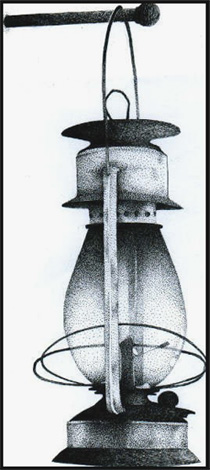
\includegraphics[scale=3]{pni30.jpg}
\end{center}
\vfill